\subsection{Пользовательские сценарии}
Для того, чтобы определить требования к нашей платформе, были проработаны пользовательские сценарии.

Прежде чем определять конкретные пользовательские сценарии, покажем высокоуровневую архитектуру системы ~\ref{sys_architecture}.

\begin{figure}
    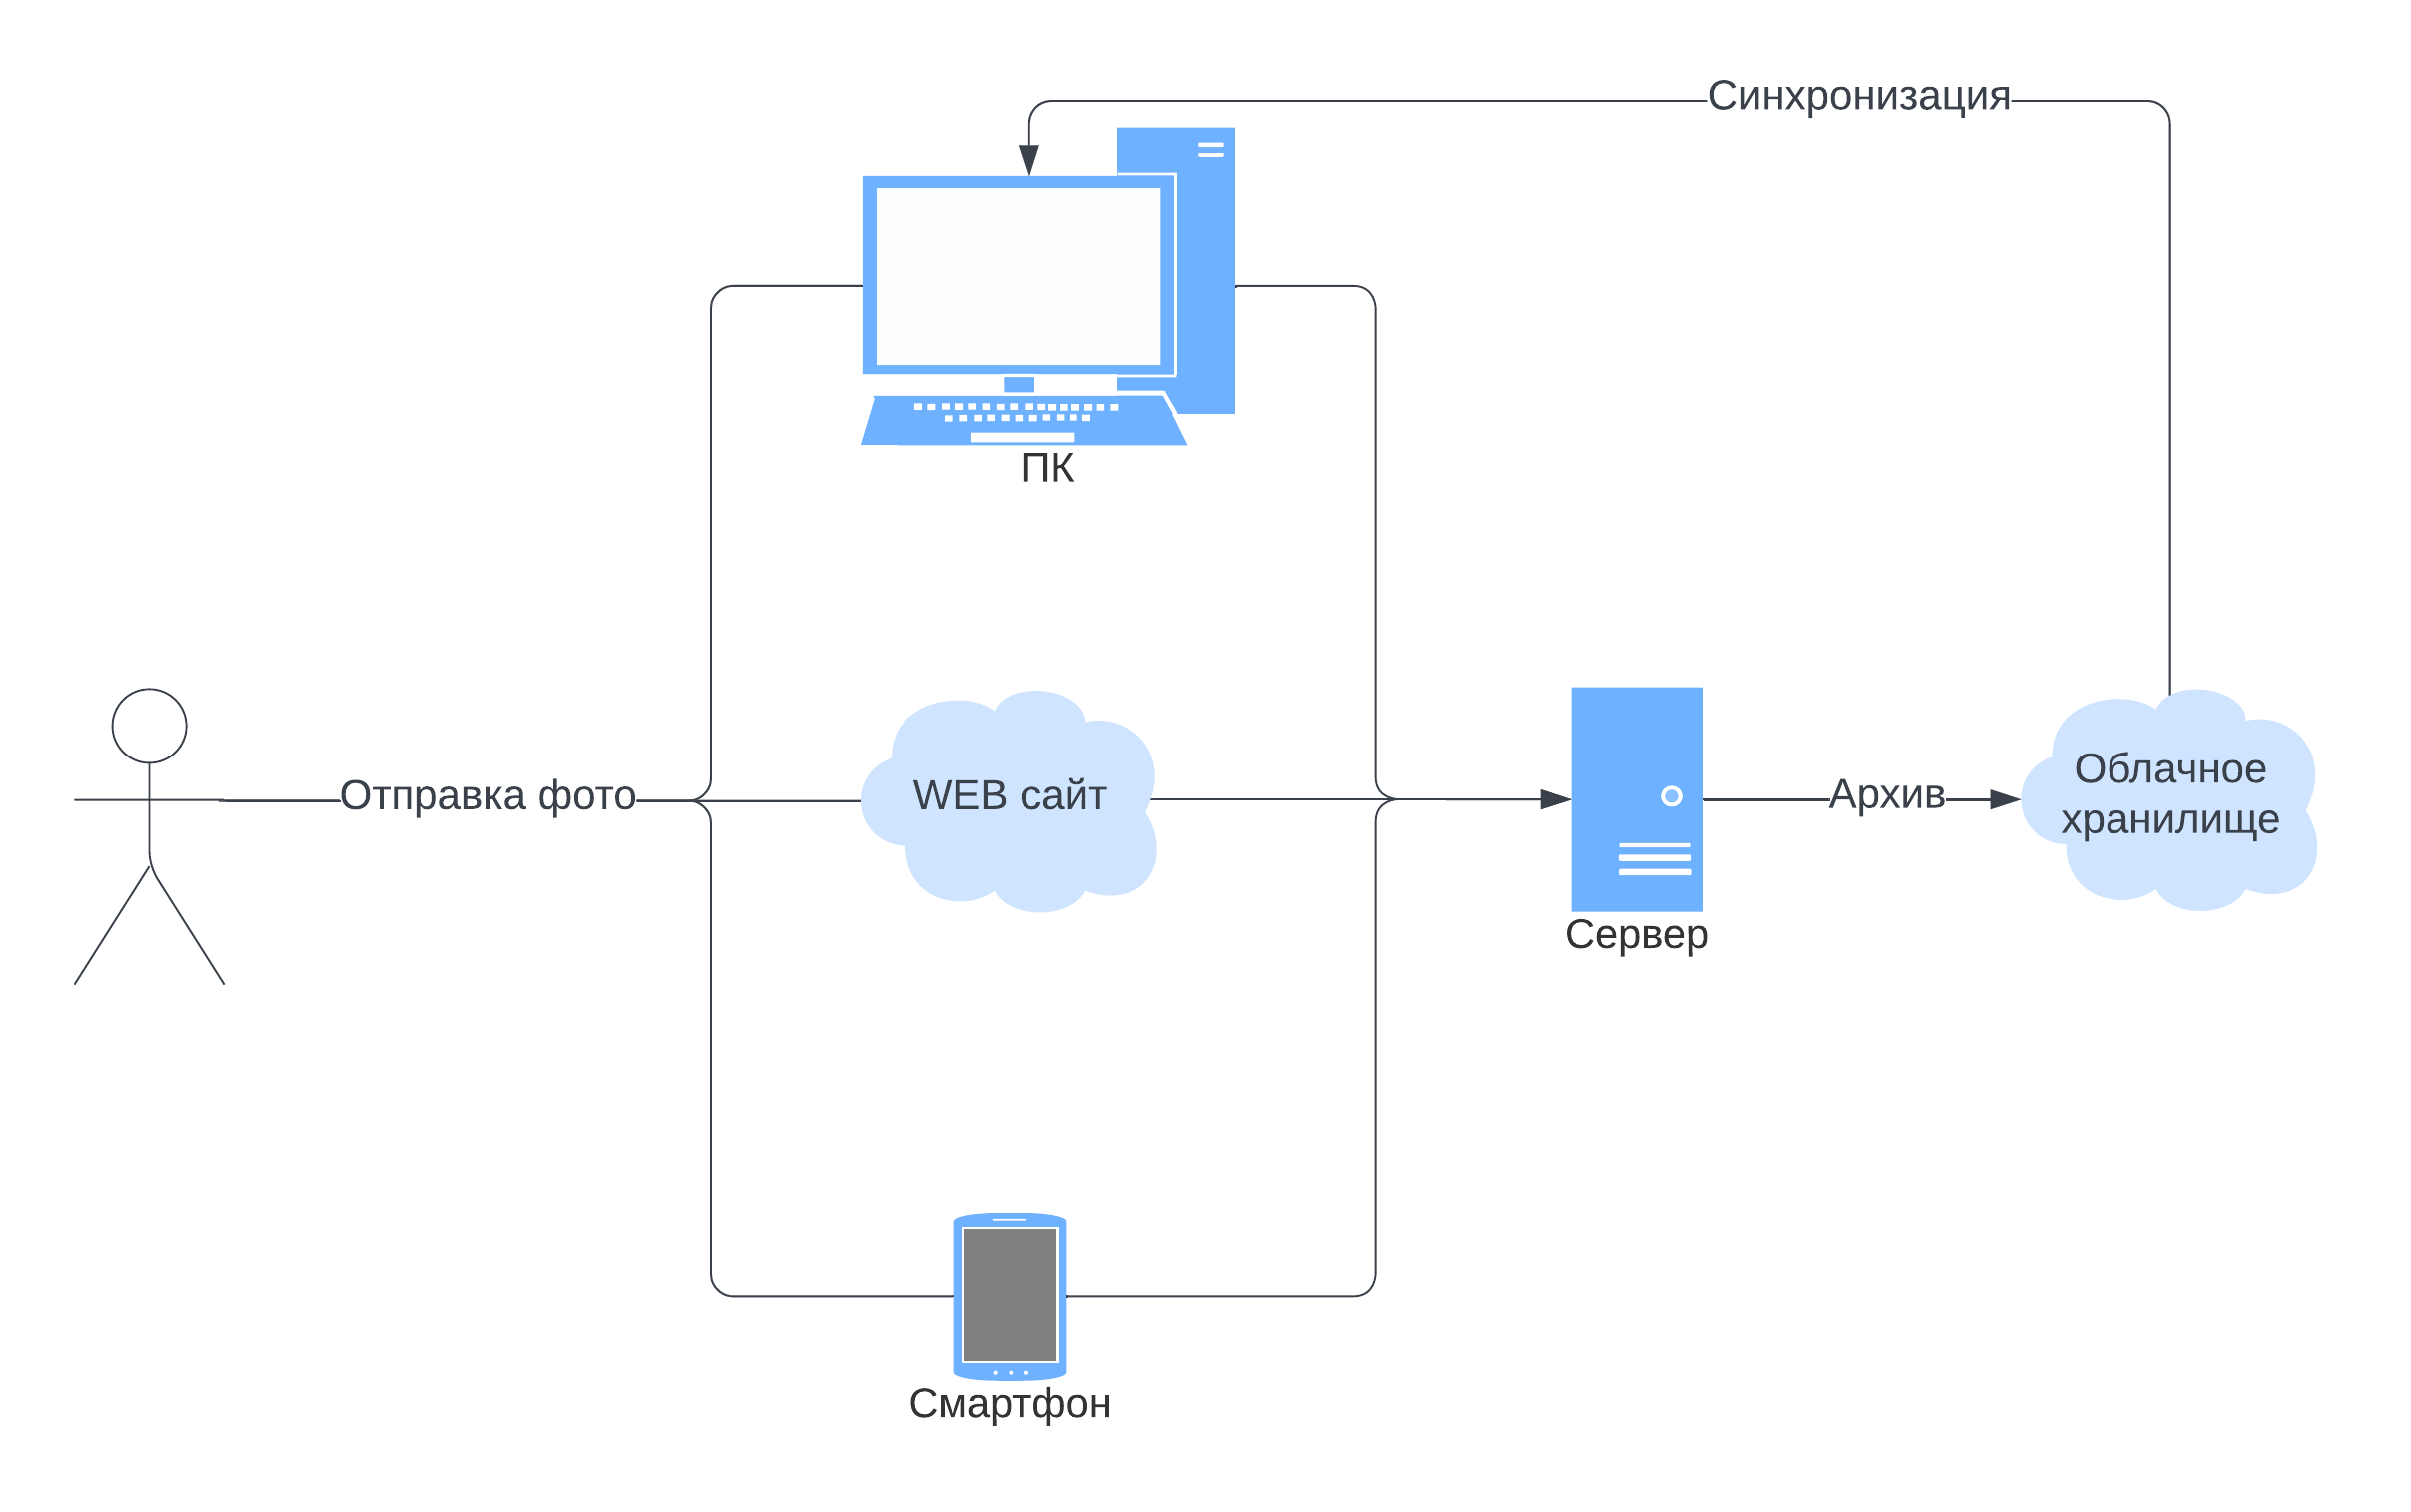
\includegraphics[scale=0.5]{img/use_cases/architecture.png}
    \caption{Высокоуровневая архитектура системы}
    \label{sys_architecture}
\end{figure}

Под пользователем приложения будем подразумевать пользователь одного из типов приложения:
\begin{itemize}
    \item $WEB$ приложение;
    \item $Desktop$ приложение;
    \item мобильное приложение.
\end{itemize}

Для начала определим основные роли целевых пользователей:
\begin{itemize}
    \item Пользователь приложения;
    \item Разработчик~--- программист, занимающийся разработкой конкретных частей приложения;
    \item Архитектор~--- работник, занимающийся планированием и разработкой высокоуровневой архитектуры приложения;
    \item Администратор системы~--- специалист, отвечающий за настройку, управление и контроль работы системы;
    \item Инженер по машинному обучению~--- специалист, занимающийся разработкой моделей машинного обучения;
    \item Аналитик данных~--- специалист, занимающийся оценкой качества обучения модели, выбором подходящих метрик, а также оптимизацией процесса обучения.
\end{itemize}

\subsubsection{Авторизация пользователя}
\underline{Участники:} пользователь любого из типов приложения

\underline{Предусловие:} пользователь не авторизован

\underline{Постусловие:} пользователь авторизован в один из сервисов и предоставлен доступ к облачному хранилищу

\underline{Сценарий:}
Для авторизации с помощью $Google$ необходимо реализовать следующий сценарий, изображенный на рисунке ~\ref{auth}:

\begin{figure}
    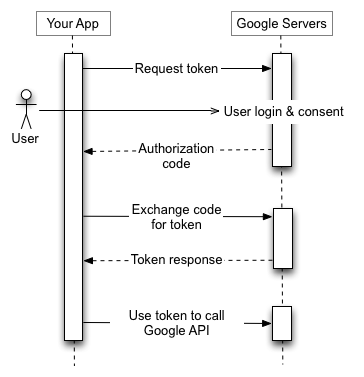
\includegraphics[scale=0.5]{img/use_cases/authorization.png}
    \caption{Сценарий сетевого взаимодействия при авторизациии пользователя \cite{OAuth_google}}
    \label{auth}
\end{figure}

По сути $Google$ делает всё сам на этапе создания сервиса внутри кода. Если приложение не видит токена для авторизации, то происходит автоматическое перенаправление на сайт авторизации. Дальнейший токен сохраняется локально.

Для замены аккаунта достаточно удалить локальный токен пользователя и перезапустить сервис $Google$. Стоит отметить, что в лучше сохранять токен для дальнейшего быстрого входа в сервис. Но так как мы разрабатываем прототип, то и этого решения будет вполне достаточно.

\subsubsection{Преобразование фотографии}
\underline{Участники:} пользователь приложения

\underline{Предусловие:} пользователь сделал фото научного текста и открыл его в приложении

\underline{Постусловие:} пользователь получает готовый \LaTeX\; код текста, полученного на изображении в виде архива из исходного кода и $pdf$ файла

\underline{Сценарий:}
\begin{itemize}
    \item Производится автоматическая коррекция перспективы фотографии
    \item Производится автоматическое сегментация текста на абзацы
    \item С приложения на сервер отправляется изображение, а также таблица с координатами начала и конца абзацев
    \item С сервера на приложение отправляется таблица с найденными формулами
    \item Пользователь проверяет правильность распознования формул и вносит коррективы
    \item Приложение отправляет на сервер таблицу с финальными формулами
    \item Сервер загружает архив с \LaTeX\; кодом и $pdf$ файлом в $Google\;Drive$, а также отсылает его пользователю
    \item $Desktop$ приложение обновляет папку $Google\;Drive$ и загружает в локальное хранилище последний архив
\end{itemize}

При необходимости пользователь может корректировать точки перспективы, а также точки абзацев на изображении.

\subsubsection{Преобразование файла формата .pdf}
\underline{Участники:} пользователь приложения

\underline{Предусловие:} пользователь загрузил файл научного текста в формате $.pdf$ в приложение

\underline{Постусловие:} пользователь получает готовый \LaTeX\; код текста, полученного на изображении в виде архива из исходного кода и $pdf$ файла

\underline{Сценарий:}
В случае с $.pdf$ файлом мы предполагаем, что нет необходимости корректировать перспективу.
\begin{itemize}
    \item Производится автоматическое сегментация текста на абзацы
    \item С приложения на сервер отправляется изображение, а также таблица с координатами начала и конца абзацев
    \item С сервера на приложение отправляется таблица с найденными формулами
    \item Пользователь проверяет правильность распознования формул и вносит коррективы
    \item Приложение отправляет на сервер таблицу с финальными формулами
    \item Сервер загружает архив с \LaTeX\; кодом и $pdf$ файлом в $Google\;Drive$, а также отсылает его пользователю
    \item $Desktop$ приложение обновляет папку $Google\;Drive$ и загружает в локальное хранилище последний архив
\end{itemize}

\subsubsection{Контроль обучения классификатора}

Так как самая важная часть системы (распознование текста) реализуется на основе нейросетевых алгоритмов (о чем будет подробно рассказно позже), важно контролировать процесс обучения.
Для этого необходимо иметь доступ к метрикам модели, а также обновлять обучающие наборы данных, проводить тестирование модели на новых данных, проводить валидацию в процессе обучения.

Важно быть уверенным в том, что модель не переобучена и способна обощать данные.

Для этих целей очень хорошо подходит платформа $\textit{Weights \& Biases}$ \cite{wandb}

\underline{Участниики:} аналитик данных

\underline{Предусловие:} сууществует рабочая система, обученная модель

\underline{Постусловие:} выводится информация об обучении модели

\underline{Сценарий:}

\begin{itemize}
    \item Пользователь заходит на веб-сайт $wandb$ \cite{wandb};
    \item Пользователь выбирает интересующую его версию модели; 
    \item Платформа выводит всю информацию о модели.
\end{itemize}

\subsubsection{Замена нейросетевых моделей}

Необходимо предусмотреть возможность замены одной модели на другую. Это является важным требованием к системе, поскольку позволяет улучшать эффективность и точность работы всей системы:
\begin{itemize}
    \item Это дает возможность адаптировать систему под изменяющиеся условия. Если модель устаревает или не удовлетворяет требованиям, необходимо иметь возможность быстро ее заменить;
    \item Это позволяет снизить затраты на разработку и поддержку системы. Вместо разработки или поддержки своей модели, можно заменить текущую модель на готовое открытое решение;
    \item Это повышает гибкость системы. При изменении требований к системе, текущая модель может не удовлетворять новым требованиям.
\end{itemize}

\underline{Участники:} инженер по машинному обучению, разработчик системы, аналитик данных

\underline{Предусловие:} существует система

\underline{Постусловие:} существует рабочая система, удовлетворяющая текущим требованиям

\underline{Сценарий:}

\begin{itemize}
    \item Инженер по машинному обучению разрабатывает новую модель или находит открытое решение;
    \item Разработчик системы встраивает новую модель в систему;
    \item Аналитик проверяет работоспособность модели, а также удовлетворение модели текущим требованиям;
    \item По результатам проверки:
        \begin{itemize}
            \item в случае удовлетворения требованиям старая модель заменяется на новую;
            \item в случае неудовлетворения требованиям цикл повторяется.
        \end{itemize}
\end{itemize}